\documentclass[tikz,border=5pt]{standalone}
\usepackage[UTF8]{ctex}
\usepackage{amsmath,amssymb}
\usetikzlibrary{arrows.meta,calc,angles,quotes,patterns,decorations.pathmorphing}
\definecolor{field}{HTML}{176B9B}
\definecolor{force}{HTML}{B64B32}
\tikzset{>=Latex,line width=.8pt,every node/.style={font=\small},field/.style={color=field},force/.style={color=force},body/.style={draw=black,fill=blue!5},ghost/.style={dashed,gray},labelbox/.style={fill=white,inner sep=1.2pt}}
\begin{document}
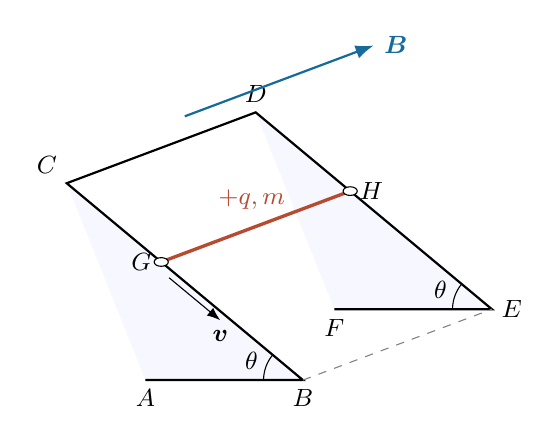
\begin{tikzpicture}
\coordinate(A)at(-2,0);\coordinate(B)at(0,0);\coordinate(C)at(-3,2.5);
\coordinate(D)at(-.6,3.4);\coordinate(E)at(2.4,.9);\coordinate(F)at(.4,.9);
\coordinate(G)at(-1.8,1.5);\coordinate(H)at(.6,2.4);
\fill[blue!3](A)--(B)--(C)--cycle;\fill[blue!3](F)--(E)--(D)--cycle;
\draw[thick](A)--(B)--(C)--(D)--(E)--(F);
\draw[ghost](B)--(E);\draw[very thick,force](G)--(H);
\draw[fill=white](G)ellipse(.09 and .055);\draw[fill=white](H)ellipse(.09 and .055);
\foreach\v/\p in{A/below,B/below,C/above left,D/above,E/right,F/below,G/left,H/right}\node[\p]at(\v){$\v$};
\draw[->,field,thick](-1.5,3.35)--(.9,4.25)node[right]{$\boldsymbol B$};
\draw[->](-1.7,1.3)--(-1.05,.76)node[below]{$\boldsymbol v$};
\draw(-.5,0)arc(180:140.2:.5);\node[left]at(-.45,.25){$\theta$};
\draw(1.9,.9)arc(180:140.2:.5);\node[left]at(1.95,1.15){$\theta$};
\node[force,above]at(-.65,2.05){$+q,m$};
\end{tikzpicture}
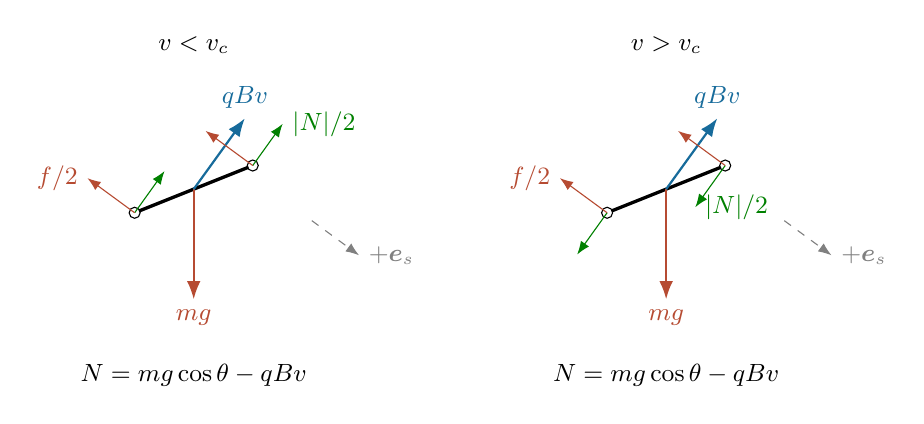
\begin{tikzpicture}
\foreach\x/\n/\sign in{0/{v<v_c}/1,6/{v>v_c}/-1}{
\begin{scope}[xshift=\x cm]
\coordinate(G)at(-.75,-.3);\coordinate(H)at(.75,.3);
\draw[very thick](G)--(H);
\foreach\v in{G,H}\draw[fill=white](\v)circle(.07);
\draw[->,force,thick](0,0)--(0,-1.4)node[below]{$mg$};
\draw[->,field,thick](0,0)--(.65,.9)node[above]{$qBv$};
\draw[->,green!50!black](G)--++({.38*\sign},{.53*\sign});
\draw[->,green!50!black](H)--++({.38*\sign},{.53*\sign})node[right]{$|N|/2$};
\draw[->,force](G)--++(-.6,.44)node[left]{$f/2$};
\draw[->,force](H)--++(-.6,.44);
\draw[->,ghost](1.5,-.4)--(2.1,-.84)node[right]{$+\boldsymbol e_s$};
\node[above]at(0,1.6){$\n$};
\node[below]at(0,-2.1){$N=mg\cos\theta-qBv$};
\end{scope}}
\end{tikzpicture}
\begin{tikzpicture}
\draw[->](0,0)--(5.2,0)node[right]{$v/v_c$};
\draw[->](0,-2.8)--(0,2.8)node[above]{归一化量};
\draw[field,thick](0,1.5)--(4.5,-3);
\draw[force,thick](0,1.5)--(1.5,0)--(4.5,3);
\draw[ghost](1.5,0)--(1.5,1.5);\node[below]at(1.5,0){$1$};
\node[left]at(0,1.5){$1$};
\node[field,right]at(3,-1.3){$N/(mg\cos\theta)$};
\node[force,labelbox]at(2.8,2.9){$f/(\mu_0mg\cos\theta)$};
\end{tikzpicture}
\begin{tikzpicture}[x=1.4cm,y=.65cm]
\draw[->](0,0)--(5.6,0)node[right]{$bt$};
\draw[->](0,0)--(0,5.8)node[above]{$v/v_c$};
\draw[field,thick,domain=0:.287682,samples=30]plot(\x,{3*(exp(\x)-1)});
\draw[force,thick,domain=.287682:5,samples=80]plot(\x,{5-4*exp(-(\x-.287682))});
\draw[ghost](0,5)--(5,5)node[right]{$v_\infty/v_c=5$};
\draw[ghost](.287682,0)--(.287682,1);
\fill(.287682,1)circle(2pt);\node[right]at(.45,.7){$t_c$};
\node[below]at(2.7,-.8){示例 $\theta=45^\circ,\ \mu_0=1/4$};
\end{tikzpicture}
\end{document}
